%!TEX encoding = UTF-8 Unicode
%!TEX program = xelatex

\documentclass[UTF8]{ctexart}


\title{近程炮弹落点的简要分析\\ \large“合肥大炮”的计算}
\author{NAME}

\usepackage{amsmath}
\usepackage[OT2,OT1]{fontenc}
\usepackage{siunitx}
\usepackage{xfrac}

\newcommand\cyr
{
	\renewcommand\rmdefault{wncyr}
	\renewcommand\sfdefault{wncyss}
	\renewcommand\encodingdefault{OT2}
	\normalfont
	\selectfont
}
\DeclareTextFontCommand{\textcyr}{\cyr}
\def\cprime{\char"7E }
\def\cdprime{\char"7F }
\def\eoborotnoye{\char’013}
\def\Eoborotnoye{\char’003}

\renewcommand{\vec}[1]{\boldsymbol{#1}} % Uncomment for BOLD vectors.

\begin{document}

	\maketitle
	
	\begin{abstract}
	本文通过对炮弹的受力分析以及计算机运算,对地球上发射的近程炮弹的落点进行了仿真模拟.在受力分析的过程中考虑了空气阻力、地球自转等的影响,能够较快速地计算出在一定初速度下炮弹打到指定坐标所需的瞄准角,并对不同的发射参数进行简单的分析.
	\\
	\textbf{关键词}:炮弹落点、仿真模拟
	\end{abstract}
	
	\section{简介}
	根据指定的要求,我们从合肥(坐标为 \ang{31;51;49}N \ang{117;16;46}E)发射一颗炮弹打到池州(坐标为 \ang{30;39;22}N \ang{117;29;20}E)\footnote{数据来自 Wikipedia.}.为了方便计算,我们首先指定某种特定的炮弹,并在之后对其进行分析.最终,我们需要找出初速度、瞄准角与落点的关系,并且给出能够成功打到池州的值(误差在半径 \SI{25}{m} 圆内).
	
	\section{模型假设}
	为了方便计算,使模型更加简洁,我们进行如下假设:
		\begin{enumerate}
			\item 由于合肥到池州距离(由坐标计算得约为 \SI{133}{km})远小于地球过赤道截面周长,所以忽略地球作为椭球体所带来的影响.
			\item 由于炮弹飞行时间远小于地球公转周期,所以可以忽略地球公转带来的影响.
			\item 不考虑两地海拔高度的变化,且假设飞行过程中不会有任何因素(如障碍物、军方拦截等)阻止炮弹飞行;空气与地球相对静止,无风等因素的作用.
			\item 不考虑不同经纬点上重力加速度 $g$ 的变化,只考虑海拔高度给 $g$ 带来的变化.
			\item 假设我们发射的炮弹质量为 \SI{100}{kg},口径为 \SI{203}{mm},阻力系数 $C_D$ 为 0.04.
		\end{enumerate}
	\section{模型建立}
	由于地球处于自转之中,我们将 $t=0$(炮弹开始发射)时的地球作为惯性系,将炮弹飞行时正在自转中的地球作为非惯性系.下面将以合肥坐标为原点,合肥所在地指向赤道方向的经线的切线为 $x$ 轴,合肥所在地指向东的纬线的切线为 $y$ 轴,合肥指向地心方向的反方向为 $z$ 轴,建立地表坐标系.
		\subsection{受力分析}
		炮弹飞行时,在非惯性系中,可以认为炮弹受到了四个力的作用.它们分别是万有引力、惯性离心力、空气阻力、科里奥利力.下面分别对这四个力进行分析.
			\subsubsection{万有引力}
			由于我们不考虑经纬度的影响,由万有引力公式,我们可以推得重力加速度与离地高度的关系为:
			$$ g(h) = \frac{g(h = 0)}{(1 + h/R_0)^2} $$
			其中 $R_0$ 为地球半径.设 $g(h=0)$ 为标准重力 \SI[per-mode=fraction,fraction-function=\sfrac]{9.80665}{\metre\per\square\second}.
			则最终得到炮弹的万有引力的表达式:
			$$ G=m(\frac{g(h = 0)}{(1 + h/R_0)^2}) $$
			力方向沿 $z$ 轴向下.
			\subsubsection{惯性离心力}
			惯性离心力的公式为:
			$$ \vec{f_c} = -m\vec{\omega} \times (\vec{\omega} \times \vec{r}') $$
			其中 $\vec{\omega}$ 为地球自转角速度,取 \SI[per-mode=fraction,fraction-function=\sfrac]{7.292e-5}{\radian\per\second},$\vec{r}'$ 为炮弹在非惯性系中的位矢.
			\subsubsection{空气阻力}
			在空气中运动时炮弹的速度较大,我们可以使用压差阻力公式:
			$$F_D=\frac{1}{2}C_D\rho v^2S$$
			其中 $F_D$ 为阻力,方向与运动方向相反,$\rho$ 为流体密度(此处即空气密度),$v$ 为流体相对物体的速度,$S$ 为垂直速度方向的物体横截面积.空气密度使用 ISO 发布的国际标准大气模型(International Standard Atmosphere,ISA)进行计算.
			\subsubsection{科里奥利力}
			科里奥利力的公式为:
			$$\vec{f_{cor}}=-2m\vec{\omega}\times \vec{v}'$$
			其中 $\vec{v}'$ 为炮弹在非惯性系中的速度.
		\subsection{建立方程}
		设初速度为 $v_0$,仰角为 $\theta$,与正北方向的方位角为 $\alpha$,合肥的纬度为 $\delta$. 由上述受力分析,我们可以列出各物理量在 $x$, $y$, $z$ 三个方向的标量式.
		$$\begin{cases}
			x(0)=0\\
			y(0)=0\\
			z(0)=0\\
			\dot x(0)=-v_0\cos\theta\cos\alpha\\
			\dot y(0)=v_0\cos\theta\sin\alpha\\
			\dot z(0)=v_0\sin\theta\\
			m\ddot x(t)=F_{Dx}+f_{corx}+f_{cx}\\
			m \ddot y(t)=F_{Dy}+f_{cory}+f_{cy}\\
			m\ddot z(t)=G_z+F_{Dz}+f_{corz}+f_{cz}\\
			\omega_x=-\omega\cos\delta\\
			\omega_y=0\\
			\omega_z=\omega\sin\delta
		\end{cases}$$
		将惯性离心力与科里奥利力的矢量式转换为标量式并代入后,三个方向的加速度式子如下.
		$$\begin{cases}
		\ddot x(t) = \sfrac{F_{Dx}}{m} + 2\omega_z v_y + \omega_x \sum \omega r - \omega^2x\\
		\ddot y(t) = \sfrac{F_{Dy}}{m} + 2\omega_x v_z - 2\omega_z v_x + \omega_y \sum \omega r - \omega^2y\\
		\ddot z(t) = g_z + \sfrac{F_{Dz}}{m} - 2\omega_x v_y + \omega_z \sum \omega r - \omega^2z
		\end{cases}$$
		其中 $\sum \omega r = \omega_x x + \omega_y y + \omega_z z$.
	\section{模型计算}
	我们采用 Python 语言对此模型进行模拟计算. Python 第三方的 scipy, numpy 等模块可以帮助我们快速编写此类科学计算程序.
	
	取 $\Delta t = $ \SI{0.01}{s} 进行模拟,在每次经过长度为 $\Delta t$ 的时间后,对炮弹的加速度、速度与位移进行迭代. 令模拟函数返回落点距离目标坐标的距离的平方,使用 scipy 中的最优化算法对模拟函数求其最小值,得到在 $v_0 = $ \SI[per-mode=fraction,fraction-function=\sfrac]{1500}{\metre\per\second} 时仰角与方位角分别为 $\theta = $ \ang{67.8234}, $\alpha = $ \ang{170.6826}(保留四位小数).此时距离目标距离的平方为 \SI{0.2475}{\meter\squared},符合误差在 \SI{25}{m} 之内的要求.
	\begin{figure}[h]
		\centering
		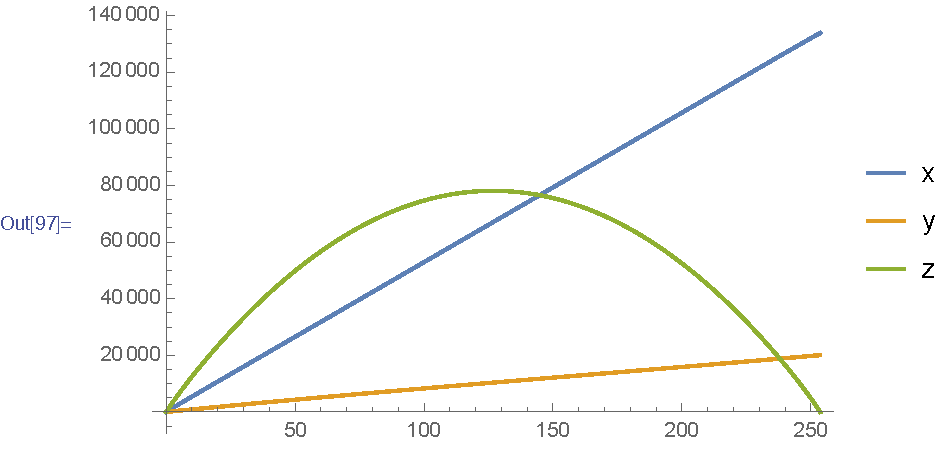
\includegraphics[height=0.1\textheight]{xyz.pdf}
		\caption{$x$, $y$, $z$ 随 $t$ 变化图像}
		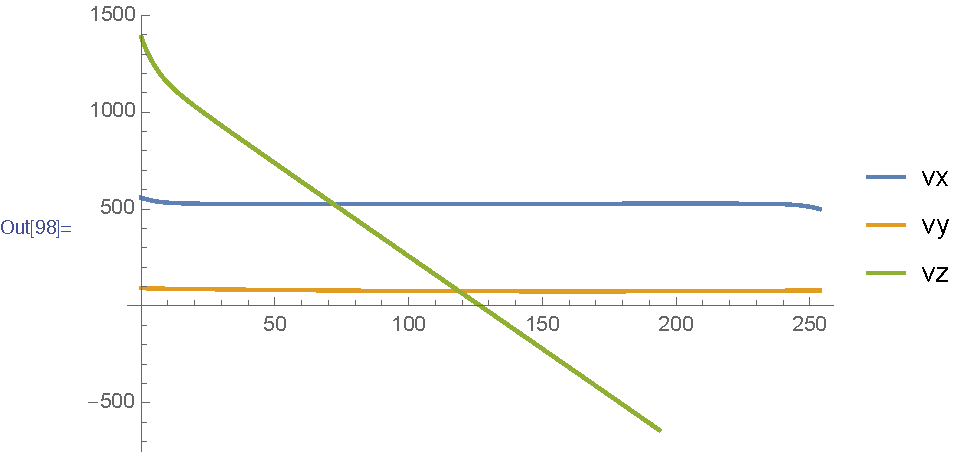
\includegraphics[height=0.1\textheight]{vxvyvz.pdf}
		\caption{$v_x$, $v_y$, $v_z$ 随 $t$ 变化图像}
		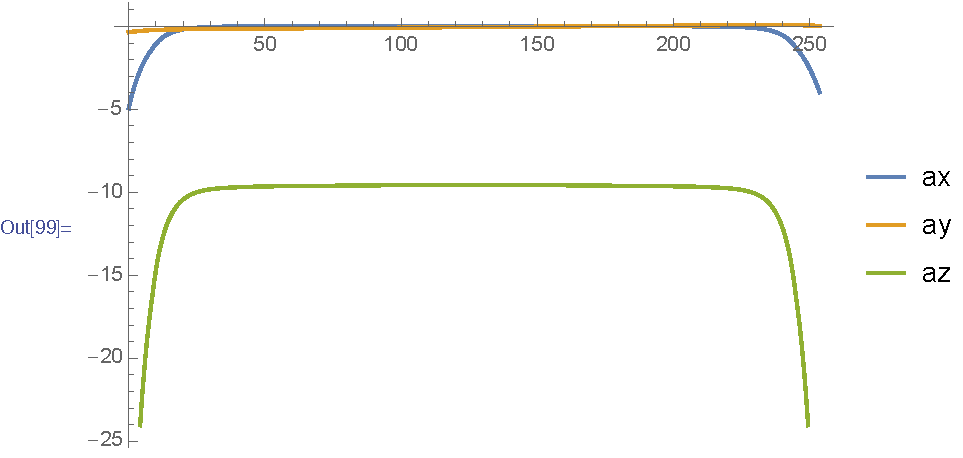
\includegraphics[height=0.1\textheight]{axayaz.pdf}
		\caption{$a_x$, $a_y$, $a_z$ 随 $t$ 变化图像}
	\end{figure}
	
	\section{结果分析}
		\subsection{可行的最小速度}
		在上述计算中我们可以发现,我们的结果是在给定初速度的条件下求出的,那么最小需要的初速度是多少?当 $v_0 = $  \SI[per-mode=fraction,fraction-function=\sfrac]{1000}{\metre\per\second} 时,模拟函数的最小值(最接近目标的落点)极大,表明此时炮弹根本打不到目标点.
		我们可以使用二分法计算最小速度. 在多次迭代后,算得最小速度为 $v_0 = $  \SI[per-mode=fraction,fraction-function=\sfrac]{1305}{\metre\per\second},此时落地点符合误差要求.
		\subsection{精度分析}
		在计算过程中可以发现,参数的精度对结果影响极大. 在 $v_0 = $ \SI[per-mode=fraction,fraction-function=\sfrac]{1500}{\metre\per\second} 处,我们对仰角、方位角舍入不同的位数,就可以发现其对结果的巨大影响.
		
		\begin{center}
			\begin{tabular}{|c|c|c|}
				\hline $\theta (°)$&$\alpha (°)$&结果(距离的平方)\\
				\hline 68&171&1289500.14716\\
				\hline 67.8&170.7&12677.2074011\\
				\hline 67.82&170.68&237.375136518\\
				\hline 67.823&170.683&7.78185476064\\
				\hline 67.8234&170.6826&0.247537689881\\
				\hline
			\end{tabular}
		\end{center}
		
		尽管保留两位小数的情况下就已经符合最大误差距离为 $25$ m 的要求,但从上表可见角度的精度对结果的极大影响. 在现实中精度不一定能达到指定的要求,在精度不足的情况下,炮弹很难精准地击中目标.
	\section{总结}
	本文建立了一种较简单的物理模型,在指定条件下对炮弹的落点进行了计算. 在现实生活中,还有其他的因素(例如风速)会对炮弹落点带来影响. 在已知具体受力情况的基础上,此模型可以进行扩展. 间接地,此模型也表明了初始状态的误差对结果带来的极大影响.
	\section{参考文献}
		\begin{enumerate}
			\item {\cyr l.n}.雷申科等. 外弹道学[M].北京:国防工业出版社,2000.
			\item Farrar C I, Leeming D W. 弹道基础[J].北京:兵器工业出版社,1990.
			\item 杨维纮. 力学与理论力学(上册)[J].北京:科学出版社,2008.
		\end{enumerate}
\end{document}
